\section{Background - IRT Parameter Estimation}
In educational measurement, a common goal is to quantify the knowledge of students from the results of some assessment. In a classroom setting, grades are typically assigned based on the percentage of questions answered correctly by a student assignments. The letter grades assigned from these percentages can serve as a naive measure of student knowledge; ``A'' students have completely mastered the material, ``B'' students have a good grasp of material, ``C'' students are fairly average, and ``D'' and ``F'' students have significant gaps in their knowledge.

The practice of evaluating student ability purely from a raw percentage score is known as true score theory \parencite{thissen} \cite{thissen} ~\textcite{thissen}. But there are clear issues with this approach. Not all questions on an exam or homework assignment is created equally: some questions are easier, and some more difficult. Consider a scenario where two students both answer 17 out of 20 questions correctly on a test for a raw score of $85\%$. But if Student A answered questions 1, 8, and 9 wrong while Student B answered 4, 17, and 20 incorrectly, it is not likely that that Student A and Student B possess the same level of knowledge. For example, questions 1, 8, and 9 could be much more difficult than questions 4, 17, and 20. Additionally, the two sets of problems could cover different types of material. True score theory does not account for either of these situations, and naively quantifies the knowledge of Student A and Student B as equal.

More sophisticated methods have been studied which attempt to more accurately quantify student learning. Cognitive Diagnostic Models (CDM) (TODO: citation) aim to classify whether students possess mastery of a given skill or not. This discrete classification can be useful in determining whether or not a student meets a prerequisite, or deciding whether or not they are ready to move on to the next level of coursework. We focus instead on Item Response Theory, where student knowledge is assumed to be continuous.

\subsection{Item Response Theory}
Item Response Theory (IRT) is a field of quantitative psychology which uses statistical models to model student ability \cite{lord1968}. These models often give the probability of a question being answered correctly as a function of the student's ability. In IRT, it is assumed that each student, indexed by $j$, possesses some continuous latent ability $\theta_j$. The term ``latent ability'' is synonymous with ``knowledge''or ``skill.'' Often, it is assumed that amongst the population of students, $\theta_j \sim \mathcal{N}(0,1)$ \cite{thissen}. 

In this work, we often consider the case where each student has multiple latent abilities. For example, in the context of an elementary math exam, we may wish to measure the four distinct skills ``add'', ``subtract'', ``multiply'', and ``divide.'' This scenario is referred to as multidimensional item response theory, and we write the set of student $j$'s $K$ latent abilities as a vector $\Theta_j = (\theta_{1j}, \theta_{2j}, \ldots, \theta_{Kj})^\top$. It is then assumed that the latent abilities of students follow some multivariate Gaussian distirbution, $\mathcal{N}(0, \Sigma)$. For simplicity, the covariance matrix $\Sigma$ is often taken to be the identity matrix, making each latent skill independent of one another.

Note that $\Theta_j$ is not directly observable in any way. Instead, a common goal is to infer student's knowledge $\Theta_j$ from on their responses on some assessment containing $n$ questions, referred to as items. A student's set of responses can be written as a binary $n$-dimensional vector $U_j = (u_{1j}, u_{2j}, \ldots, u_{nj})^\top$, where 
\begin{equation}
  u_{ij} = \begin{cases} 1 & \text{if student } j \text{ answers item } i \text{ correctly} \\0 & \text{otherwise} \end{cases} 
\end{equation}
IRT models aim to model the probability of a student answering a particular question correctly, so that the probability of student $j$ answering item $i$ correctly is given by some function of $\Theta_j$:
\begin{equation}
  P(u_{ij} = 1 | \Theta_j) = f(\Theta_j; V_i)
\end{equation}
where $V_i$ is a set of parameters associated with item $i$. In general, $f:\R^K \to [0,1]$ is some continuous function which is strictly increasing with respect to $\Theta_j$.

\begin{figure}[h]
  \centering
  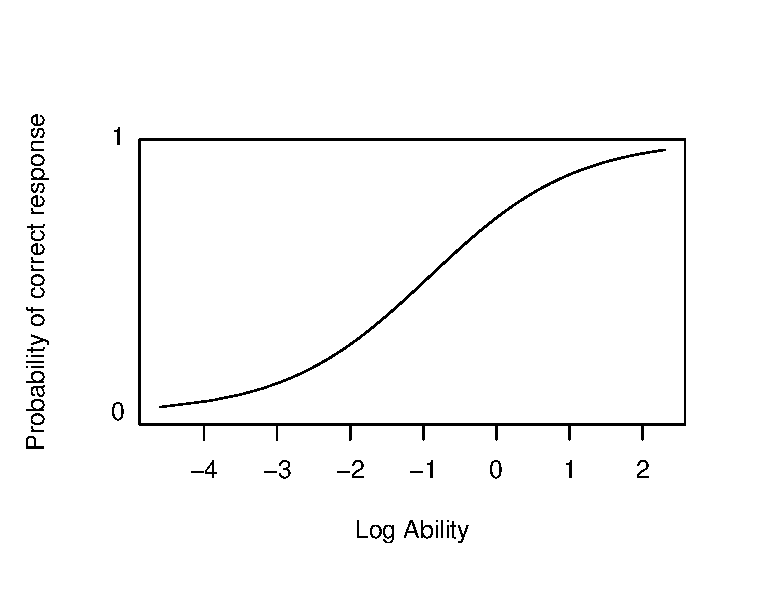
\includegraphics[width=.6\textwidth, angle=90]{img/logistic_1param_icc.eps}
  \caption{An item characteristic curve visualizes the relation between a student's ability and the probability of answering an item correctly.}
  \label{fig:icc}
\end{figure}

In the following sections, we describe various candidates for the function $f$. Though each is presented in the context of single-dimensional IRT ($K = 1$), they can all be easily adapted to higher dimensions.

\subsubsection{Rasch Model}
One of the first models was proposed by Georg Rasch in 1960. Rasch asserted that the probability of a student answering an item correctly is a function of the ratio $\xi / \d$, where $\xi > 0$ represents the student's knowledge, and $\d > 0$ quantifies the difficulty of an item. Consider the $\frac{\xi}{\xi + \d} = \frac{1}{1 + \d / \xi}$ and note that $\frac{\xi}{\xi + \d} \to 1$ as $\xi \to \infty$. After the reparametarization $\xi = e^{\theta}$ and $\d = e^{b}$, we arrive at the 1-Parameter Logistic Model, often referred to as the Rasch Model.
\begin{equation}
  P(u_{ij} = 1 | \theta_j; b_i) = \frac{1}{1 + e^{b_i - \theta_j}}
  \label{eq:1pl}
\end{equation}

Note that $\theta \in \R$ and $b \in \R$ still represent student ability and item difficulty, respectively. We can interpret the difficulty parameter $b$ as a threshold: when $\theta = b$, then the student has a $50\%$ chance of answering the question correctly. A plot of Equation \ref{eq:1pl} for a fixed item (fixed $b_i$) is shown in Figure \ref{fig:icc}. The horizontal axis represents $\log \theta$, and the vertical axis represents $P(u_{ij} = 1 | \theta, b_i)$. This type of graph is often referred to as an item characteristic curve (ICC).

\subsubsection{Normal Ogive Model}
A slightly more sophisticated method for measuring student performance is the normal ogive model. We introduce a discrimination parameter, $a_i$, which quantifies the capability of item $i$ in distinguishing between students who have / have not mastered the knowledge concept $\theta$ \cite{thissen}. In other words, $a_i$ tells \textit{how much} of skill $\theta$ is required to answer item $i$ correctly. 

The normal ogive model give the probability of student $j$ answering item $i$ correctly as
\begin{equation}
  P(u_{ij} = 1 | \theta_j; a_i, b_i) = \frac{1}{\sqrt{2\pi}} \int_{-a_i \theta_j + b_i}^\infty e^{\frac{-z^{2}}{2}}dz
  \label{eq:ogive}
\end{equation}
Note the similarity between Equation \ref{eq:ogive} and the cumulative distribution function for a Gaussian distribution. The normal ogive model is popular among statisticians for this reason, but can be difficult to use for parameter estimation. 

\subsubsection{2-Parameter Logistic Model}
The model which this work focuses on most is the 2-parameter logistic (2PL) model. Like the normal ogive model, the 2PL model uses both the discrimination and difficulty item parameters. The probability of student $j$ answering item $i$ correctly is given by
\begin{equation}
  P(u_{ij} = 1 | \theta_j; a_i, b_i) = \frac{1}{1 + e^{-a_i \theta_j + b_i}}
  \label{eq:2PL}
\end{equation}
Equation \ref{eq:2PL} has the same form as that of the Rasch model in Equation \ref{eq:1pl}, but adds in the discrimination parameter $a_i$. If this parameter is scaled by 1.7, then the ICC from the normal ogive model differs from that of the 2PL model by $0.001$??? **TODO: citation and number lookup**. In a sense, we can consider the 2PL model to be a very good approximation of the normal ogive model. Due to the simple form of Equation \ref{eq:2PL}, using this model makes parameter estimation much easier.

\subsubsection{Multidimensional Item Response Theory (MIRT)}
The previously described statistical models can all be extended to multidimensional latent abilities $\Theta = (\theta_1,\ldots, \theta_K)^\top$. The generalization of \ref{eq:2PL} is given by the multidimensional logistic 2-parameter (ML2P) model:
\begin{equation}
Pju_{ij} = 1 | \Theta_j; \vec{a_i}, b_i) = \frac{1}{1 + \exp\left(-\vec{a_i}^\top \Theta_j + b_i\right)} = \frac{1}{\exp\left(-\sum_{k=1}^K a_{ik} \theta_{kj} + b_i \right)}
  \label{eq:ml2p}
\end{equation}
Here, the discrimination parameters $\vec{a_i} \in \R^K$ are given as vector, where each entry $a_{ik} \in \vec{a_i}$ quantifies \textit{how much} of skill $k$ is required to answer item $i$ correctly. The ML2P model is the main focus of this thesis.

TODO: mention MDISC and how this scales

In MIRT, it is convenient to notate the relationship between skills and items with binary matrix. Define the Q-matrix (TODO: citation) $Q \in \R^{n\times K}$ so that 
\begin{equation}
  q_{ik} = \begin{cases}
    1 & \text{if item } i \text{ requires skill } k\\
    0 & otherwise
  \end{cases}.
  \label{eq:q_matrix}
\end{equation}
In real applications, the Q-matrix is annotated by an expert in the field, as it is usually possible to discern the concepts need to answer an item correctly. In relation to the ML2P model (Equation \ref{eq:ml2p}), notice that if $q_{ik} = 0$, then $a_{ik} = 0$ as well. Though experts can produce a Q-matrix for a given assessment, the matrix of discrimination parameters $(a_{ik})_{i,k}$ can not be discovered so easily.

\subsection{Parameter Estimation Methods}

\subsubsection{Maximum Likelihood Estimation}
TODO: item parameter estimation

TODO: ability parameter estimation

\subsubsection{Joint Maximum Likelihood Estimation}


\subsubsection{Marginal Maximum Likelihood Estimation}
TODO: MMLE

TODO: EM 

\subsection{Artificial Neural Networks}
In recent years, artifical neural networks (ANN) have become an increasingly popular tool for machine learning problems. Though they have been around since the 1960's (TODO: citation), GPU technology has become more accessible and modern computers are more powerful, allowing anyone interested to train a basic neural network on their machine. ANN can be applied to a diverse set of problems, including regression, classification, computer vision, natural language processing, function approximation, data generation, and more (TODO: citations).

One of the biggest critiques of ANN is their black-box nature, meaning that the decision process that a trained model uses is typically not explainable by humans. As opposed to simpler methods such as decision trees or linear regression, neural networks are not interpretable. This makes them less desirable in certain applications where researchers wish to know \textit{why} a model predicts a particular data sample the way that it does. For example, if a financial institution is using data science methods to determine whether or not to approve someone's loan, the institution should be able to explain to the customer why they were denied. Most customers will not be satisfied with ``the computer told us so,'' and there is a possibility that a black-box neural network could learn and use features such as race or gender in its prediction, which is illegal in the United States (TODO: definitely need citation or delete).

\subsubsection{Autoencoders}

\subsubsection{Variational Autoencoders}
TODO: describe probabilistic derivation of VAE (ie Kingma and Welling). Also talk about how Zhao et al (InfoVAE) show that if decoder is Gaussian, then maximizing ELBO makes the latent distribution bad - bu I've shown this isn't the case in our model, where the decoder is Bernoulli.

\end{center}
